\section{Frekvenční charakteristika}

Pro vytvoření frekvenční charakteristiky filtru byla použita funkce "signal.sosfreqz", která z dat filtru vytvoří data frekvenční charakteristiky pro daný filtr.
Tato funkce vrací pole normovaných frekvencí v rozmezí 0 - pi a pole frekvenční odezvy jako komplexní čísla.

Prvním krokem je převod normované frekvence na klasickou frekvenci.
Pro frekvenční odezvu v decibelech jsou hodnoty modulu přepočítány na decibely.
Tyto hodnoty jsou potom zobrazeny v grafu.
Frekvenční charakteristika v modulu a argumentu se liší tím že komplexní čísla odezvy jsou nejdřív převedena na modul pomocí funkce "np.abs" a argument je získán pomocí "np.angle" a graf byl vykreslen podle příkladu na \url{https://nbviewer.org/github/zmolikova/ISS_project_study_phase/blob/master/Zvuk_spektra_filtrace.ipynb}.

Lze vidět že je zde malý rozdíl mezi Butterworth a Elliptic filtrem. Přenos Elliptic filtru klesne skoro o 3dB těsně před přechodem a taky je zde zákmit v záverném směru k -40dB, zatímco Butterworth filtr nic takového nemá, takže pro tento případ by se Butterworth filtr dal považovat za lepší, protože není žádoucí aby klesal přenos v propustném směru před samotným přechodem do závěrného směru a zároveň chceme aby filtr v závěrném směru propouštěl co nejméně.
\subsection{Elliptic filtry}
\begin{figure}[H] 
	\centering
	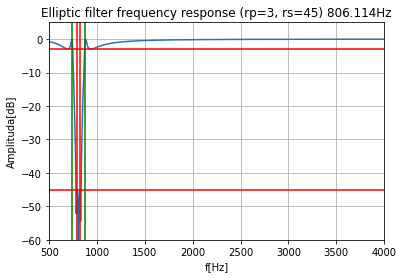
\includegraphics[scale=0.65,keepaspectratio]{Figure_10}
	\caption{Frekvenční odezva Elliptic filtru 1}
\end{figure}

\begin{figure}[H] 
	\centering
	\includegraphics[scale=0.65,keepaspectratio]{Figure_35}
	\caption{Frekvenční charakteristika Elliptic filtru 1}
\end{figure}

\begin{figure}[H] 
	\centering
	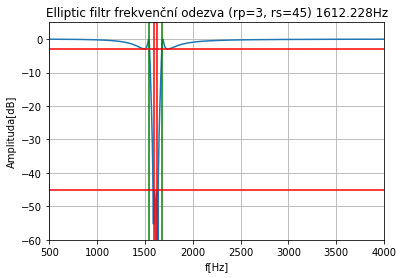
\includegraphics[scale=0.65,keepaspectratio]{Figure_11}
	\caption{Frekvenční odezva Elliptic filtru 2}
\end{figure}

\begin{figure}[H] 
	\centering
	\includegraphics[scale=0.65,keepaspectratio]{Figure_36}
	\caption{Frekvenční charakteristika Elliptic filtru 2}
\end{figure}

\begin{figure}[H] 
	\centering
	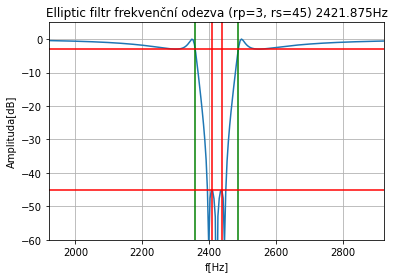
\includegraphics[scale=0.65,keepaspectratio]{Figure_12}
	\caption{Frekvenční odezva Elliptic filtru 3}
\end{figure}

\begin{figure}[H] 
	\centering
	\includegraphics[scale=0.65,keepaspectratio]{Figure_37}
	\caption{Frekvenční charakteristika Elliptic filtru 3}
\end{figure}

\begin{figure}[H] 
	\centering
	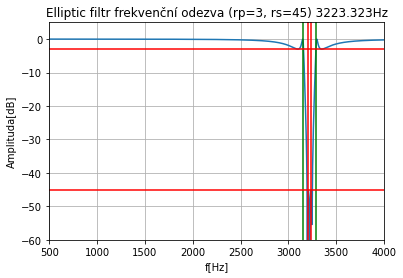
\includegraphics[scale=0.65,keepaspectratio]{Figure_13}
	\caption{Frekvenční odezva Elliptic filtru 4}
\end{figure}

\begin{figure}[H] 
	\centering
	\includegraphics[scale=0.65,keepaspectratio]{Figure_38}
	\caption{Frekvenční charakteristika Elliptic filtru 4}
\end{figure}

\subsection{Butterworth filtry}
\begin{figure}[H] 
	\centering
	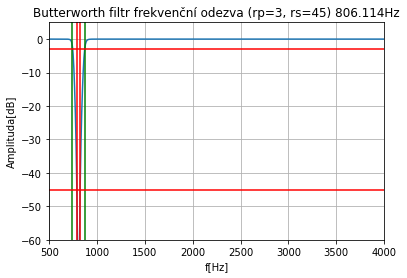
\includegraphics[scale=0.65,keepaspectratio]{Figure_14}
	\caption{Frekvenční odezva Butterworth filtru 1}
\end{figure}

\begin{figure}[H] 
	\centering
	\includegraphics[scale=0.65,keepaspectratio]{Figure_39}
	\caption{Frekvenční charakteristika Butterworth filtru 1}
\end{figure}

\begin{figure}[H] 
	\centering
	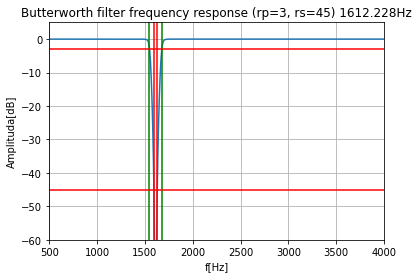
\includegraphics[scale=0.65,keepaspectratio]{Figure_15}
	\caption{Frekvenční odezva Butterworth filtru 2}
\end{figure}

\begin{figure}[H] 
	\centering
	\includegraphics[scale=0.65,keepaspectratio]{Figure_40}
	\caption{Frekvenční charakteristika Butterworth filtru 2}
\end{figure}

\begin{figure}[H] 
	\centering
	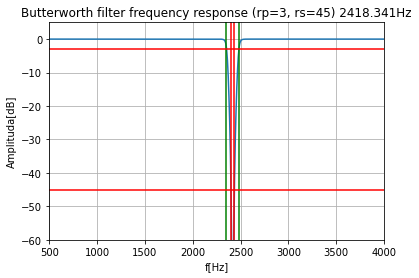
\includegraphics[scale=0.65,keepaspectratio]{Figure_16}
	\caption{Frekvenční odezva Butterworth filtru 3}
\end{figure}

\begin{figure}[H] 
	\centering
	\includegraphics[scale=0.65,keepaspectratio]{Figure_41}
	\caption{Frekvenční charakteristika Butterworth filtru 3}
\end{figure}

\begin{figure}[H] 
	\centering
	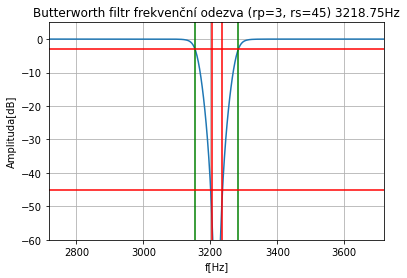
\includegraphics[scale=0.65,keepaspectratio]{Figure_17}
	\caption{Frekvenční odezva Butterworth filtru 4}
\end{figure}

\begin{figure}[H] 
	\centering
	\includegraphics[scale=0.65,keepaspectratio]{Figure_42}
	\caption{Frekvenční charakteristika Butterworth filtru 4}
\end{figure}